\pgfplotsset{compat=1.12}

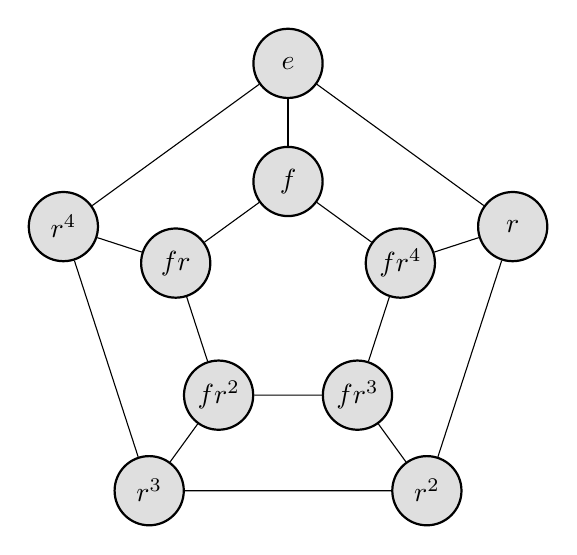
\begin{tikzpicture}[rotate=90,scale=1.5]
\tikzstyle{vertex}=[draw,thick,circle,fill=lightgray!50,minimum size=25pt,inner sep=0pt]
\def\k{360/5}
\draw (-0*\k : 1) node[vertex] (v1)  {$f$};
\draw (-0*\k : 2) node[vertex] (v2)  {$e$};
\draw (-1*\k : 1) node[vertex] (v3)  {$f r^4$};
\draw (-1*\k : 2) node[vertex] (v4)  {$r$};
\draw (-2*\k : 1) node[vertex] (v5)  {$f r^3$};
\draw (-2*\k : 2) node[vertex] (v6)  {$r^2$};
\draw (-3*\k : 1) node[vertex] (v7)  {$f r^2$};
\draw (-3*\k : 2) node[vertex] (v8)  {$r^3$};
\draw (-4*\k : 1) node[vertex] (v9)  {$f r$};
\draw (-4*\k : 2) node[vertex] (v10) {$r^4$};
\draw (v2) -- (v1);
\draw (v2) -- (v1);
\draw (v3) -- (v1);
\draw (v4) -- (v2);
\draw (v4) -- (v3);
\draw (v5) -- (v3);
\draw (v6) -- (v4);
\draw (v6) -- (v5);
\draw (v7) -- (v5);
\draw (v8) -- (v6);
\draw (v8) -- (v7);
\draw (v9) -- (v1);
\draw (v9) -- (v7);
\draw (v10) -- (v2);
\draw (v10) -- (v8);
\draw (v10) -- (v9);
\end{tikzpicture}

% This Cayley graph is taken from here
% https://beckytikz.wordpress.com/2013/09/21/some-simply-cayley-graphs/  

